\documentclass[11pt,letterpaper]{article}
\usepackage[lmargin=1in,rmargin=1in,tmargin=1in,bmargin=1in]{geometry}
\usepackage{../style/homework}
\setbool{quotetype}{true} % True: Side; False: Under
\setbool{hideans}{true} % Student: True; Instructor: False

% -------------------
% Content
% -------------------
\begin{document}

\homework{20: Due 04/24}{Okay. No hard feelings, but I hate you. Not joking. Bye.}{Gina Linetti, Brooklyn 99}

% Problem 1
\problem{10} Consider the polynomial $f(x)= x^3 (x^2 + 1) (x + 4)^2 (x - 5) (x + 8)^3$. 
	\begin{enumerate}[(a)]
	\item What is the degree of $f(x)$?
	\item How many real zeros does $f(x)$ have?
	\item How many complex zeros does $f(x)$ have?
	\item Does $f(x)$ have a maximum or a minimum? Explain. 
	\end{enumerate}



\newpage



% Problem 2
\problem{10} Determine the real quadratic polynomial that has a root at $x= 1 + 3i$ and has $y$-intercept 1.



\newpage



% Problem 3
\problem{10} Suppose that $f(x)$ is a degree five polynomial (quintic polynomial) with $f(-1)= f(2)= f(4)= f(5)= f(10)= 0$ and $f(0)= -7$. Find the polynomial $f(x)$. \pspace



\newpage



% Problem 4
\problem{10} Suppose $f(x)$ is a real quintic polynomial whose graph is given below. How many real zeros does $f(x)$ have? How many complex zeros does $f(x)$ have? Find $f(x)$. 
	\[
	\fbox{
	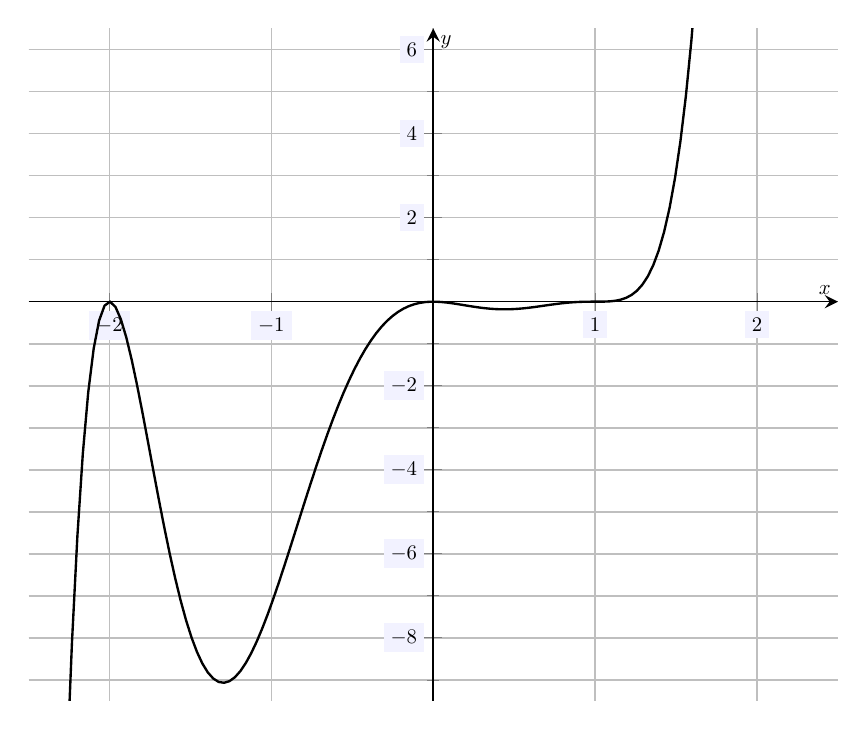
\begin{tikzpicture}[scale=1.5,every node/.style={scale=0.5}]
	\begin{axis}[
	grid=both,
	axis lines=middle,
	ticklabel style={fill=blue!5!white},
	xmin= -2.5, xmax=2.5,
	ymin= -9.5, ymax=6.5,
	xtick={-5,-4,...,5},
	ytick={-10,-8,...,10},
	minor tick = {-10,-9,...,10},
	xlabel=\(x\),ylabel=\(y\),
	]
	\addplot[line width= 0.02cm,samples=150,domain= -2.5:2.5] ({x},{0.9*x^2*(x + 2)^2*(x - 1)^3});
	\end{axis}
	\end{tikzpicture}
	}
	\]


\end{document}